\section{量化}

\begin{logicbox}[title=引言]
本节讨论如何通过量化将命题函项转变为命题。我们将介绍全称量词和存在量词的概念及符号表示,分析它们之间的逻辑关系,并探讨如何使用量化符号来表达不同类型的普遍命题,从而为理解更复杂的逻辑结构奠定基础。
\end{logicbox}

\subsection{从命题函项到命题的两种路径}

用个体常元代人个体变元,并不是从命题函项获得命题的唯一方式。通过概括或量化程序也可以得到命题。

\begin{theorembox}[title=生成命题的两种基本方法]
从命题函项生成命题有两种根本不同的方法:

\textbf{1. 列举方法(Instantiation)}:
\begin{itemize}
\item 用个体常元代入个体变元
\item 产生关于特定个体的单称命题
\item 例如:从$H(x)$得到$H(s)$(苏格拉底是人)
\item 这种方法产生具体的、特殊的陈述
\end{itemize}

\textbf{2. 概括方法(Generalization)}:
\begin{itemize}
\item 通过量词对个体变元进行约束
\item 产生关于个体集合或类别的普遍命题
\item 例如:从$H(x)$得到$(x)H(x)$(所有事物都是人)
\item 这种方法产生一般的、普遍的陈述
\end{itemize}

这两种方法体现了逻辑思维中从特殊到一般、从一般到特殊的双向运动。
\end{theorembox}

\begin{examplebox}[title=普遍命题的特征]
谓项通常不仅仅出现在单称命题中。例如,命题"每个事物是有死的"和"有些事物是漂亮的"含有谓项,但不是单称命题,因为它们不含有任何特定个体的名称。

\textbf{普遍命题的重要特征}:
\begin{itemize}
\item \textbf{非特指性}:不特别指称任何特定个体
\item \textbf{范围性}:涉及整个个体域或其子集
\item \textbf{模式性}:表达个体之间的一般模式或规律
\item \textbf{预测性}:可以对未知个体做出预测
\end{itemize}

相反,作为普遍命题,它们不特别指称任何特定个体,而是对整个个体域做出断言。
\end{examplebox}

第一个命题可以用各种不同的逻辑等价的方式表示:或者表示为"所有事物都是有死的",或者表示为:

给定不管任何个体事物,它都是有死的。

在后一种表述中,语词"它"是一个关系代词,回指该陈述中前面的语词 "事物"。用字母 $x$ ,即个体变元,代替代词"它"及其先行词,我们可以把第一个普遍命题重写为:

给定任何 $x, x$ 是有死的。

或者,用前一节所介绍的符号,我们可以写成:

给定任何 $x, M x$ 。

尽管命题函项 $M x$ 不是一个命题,但我们这里有了一个含有它的表述式,而这个表述式是命题。

\begin{theorembox}[title=全称量词的深入分析]
短语"给定任何 $x$"习惯上用符号"$(x)$"表示,称为\logicterm{全称量词}。

\textbf{全称量词的本质特征}:
\begin{itemize}
\item \textbf{约束功能}:将自由变元转换为约束变元
\item \textbf{普遍性}:表达对整个个体域的断言
\item \textbf{逻辑强度}:全称陈述比存在陈述具有更强的逻辑承诺
\item \textbf{可证伪性}:一个反例就足以证伪全称陈述
\end{itemize}

\textbf{全称量词的哲学意义}:
\begin{itemize}
\item 体现了人类认识从个别到一般的抽象能力
\item 是科学定律和数学定理的逻辑基础
\item 反映了理性思维对普遍性的追求
\item 连接经验观察与理论概括的桥梁
\end{itemize}
\end{theorembox}

上述第一个普遍命题可以完全符号化为:
$$(x)Mx$$

这个符号表达式读作:"对于所有的$x$,$x$是有死的"或"每个$x$都是有死的"。

\subsection{存在量化与全称量化}

第二个普遍命题,即"有些事物是漂亮的",也可以表达成:

至少存在这样一个事物,它是漂亮的。

在后一个表述中,语词"它"也是一个关系代词,回指语词"事物"。用个体变元 $x$ 代替代词"它"及其先行词,我们可以把第二个普遍命题重写为:

至少存在这样一个 $x, x$ 是漂亮的。

或者,我们可以用给定符号把它写成:

至少存在这样一个 $x, B x$ 。

同样,尽管 $B x$ 是一个命题函项而不是命题,但我们这里又有一个含有它的表述式,这个表述式是命题。

\begin{theorembox}[title=存在量词的深入分析]
短语"至少存在这样一个 $x$"习惯上用符号"$(\exists x)$"表示,称为\logicterm{存在量词}。

\textbf{存在量词的本质特征}:
\begin{itemize}
\item \textbf{存在承诺}:断言至少有一个个体满足给定条件
\item \textbf{弱逻辑强度}:比全称陈述更容易满足
\item \textbf{可验证性}:找到一个正例就足以验证存在陈述
\item \textbf{开放性}:不指定具体是哪个个体满足条件
\end{itemize}

\textbf{存在量词的认识论意义}:
\begin{itemize}
\item 反映了人类对世界多样性的认识
\item 是发现和探索的逻辑基础
\item 体现了可能性思维的重要性
\item 为假设和猜想提供逻辑框架
\end{itemize}
\end{theorembox}

第二个普遍命题可以完全符号化为:
$$(\exists x) B x$$

这个符号表达式读作:"存在一个$x$使得$x$是漂亮的"或"有些$x$是漂亮的"。

\begin{examplebox}[title=两种生成方法的总结]
于是我们看到,命题可以用两种方法从命题函项生成:

\textbf{1. 列举方法}:通过用个体常元代入个体变元
\begin{itemize}
\item 产生具体的单称命题
\item 例如:$H(x) \rightarrow H(s)$
\item 适用于关于特定个体的断言
\end{itemize}

\textbf{2. 概括方法}:在命题函项前面放一个量词
\begin{itemize}
\item 产生普遍的量化命题
\item 例如:$H(x) \rightarrow (x)H(x)$ 或 $(\exists x)H(x)$
\item 适用于关于个体类别的断言
\end{itemize}

这两种方法构成了谓词逻辑的基本操作,使我们能够在特殊与一般之间自由转换。
\end{examplebox}

\subsection{量化命题的真值条件}

\begin{theorembox}[title=量化命题真值条件的精确定义]
现在请考虑量化命题的真值条件:

\textbf{全称量化的真值条件}:
一个命题函项的全称量化式 $(x) M x$ 为真,当且仅当,它的所有代入例都为真;这正是普遍性的意义之所在。

\textbf{存在量化的真值条件}:
很显然,一个命题函项的存在量化式 $(\exists x) M x$ 为真,当且仅当,它至少有一个真代入例。

\textbf{个体域的假定}:
我们假定(没人会否认这一点)至少存在一个个体。这是一个非常弱但重要的假定,被称为\logicterm{存在假定}。
\end{theorembox}

\begin{examplebox}[title=量词间的逻辑关系]
在存在假定下,每个命题函项必定至少有一个代入例,这个实例或真或假。

\textbf{重要的逻辑关系}:
如果一个命题函项的全称量化式为真,那么它的存在量化式也必定为真。

\textbf{形式表示}:$(x)Mx \rightarrow (\exists x)Mx$

\textbf{直观理解}:如果每个 $x$ 都是 $M$ ,那么,如果至少存在一个事物,则这个事物是 $M$ 。

\textbf{哲学意义}:这个关系体现了从普遍到特殊的逻辑推理,是演绎推理的基础。但反向关系不成立:从存在到全称的推理是归纳性的,不具有逻辑必然性。
\end{examplebox}

\subsection{否定与量化}

到此时为止,只举了单称肯定命题作为命题函项的代入例。

\begin{theorembox}[title=否定在命题函项中的作用]
$M x$($x$ 是有死的)是一个命题函项。$M s$ 是它的一个实例,是一个单称肯定命题,即"苏格拉底是有死的"。

\textbf{否定的引入}:
但并非所有命题都是肯定的。一个人可以否认苏格拉底是有死的,即 $\sim M s$ ,"苏格拉底不是有死的"。

\textbf{否定命题函项}:
如果 $M s$ 是 $M x$ 的一个代入例,那么,$\sim Ms$可以看成是命题函项 $\sim M x$ 的一个代入例。

\textbf{概念扩展}:
因此,我们可以超出前一节所介绍的简单谓述,把我们的命题函项概念扩大到能包括否定符"$\sim$"。

\textbf{否定的重要性}:
\begin{itemize}
\item 增强了表达能力,可以表达否定性质
\item 为量词的相互转换提供了基础
\item 使逻辑系统更加完整和对称
\item 反映了思维的批判性和辨析能力
\end{itemize}
\end{theorembox}

如下所示,使用否定符可以丰富我们对量化的理解。从下述普遍命题出发:

没有任何事物是完美的。

我们可以把它解释为:

每个事物都是不完美的。

它又可以写成:

给定不管任何个体事物,它不是完美的。

它可以改写成:

给定任何 $x, x$ 不是完美的。

如果用 $P$ 符号化属性"是完美的",用刚才给出的符号(量词和否定符),我们可以把这个命题("没有任何事物是完美的")表示为 $(x) \sim P x$ 。

\subsection{量词间的逻辑关系深入分析}

现在我们可以列出并举例说明全称量化和存在量化之间的一系列重要关系。

\begin{theorembox}[title=量词对偶关系的第一组]
\textbf{第一个重要关系}:

(全称)普遍命题"每个事物都是有死的",被(存在)普遍命题"有些事物不是有死的"否定。

\textbf{符号表示}:$(x)Mx$ 被 $(\exists x)\sim Mx$ 否定。

\textbf{逻辑分析}:
\begin{itemize}
\item 这两个命题是矛盾关系,不能同时为真,也不能同时为假
\item 一个为真当且仅当另一个为假
\item 这体现了全称断言的可证伪性:一个反例就足以推翻全称命题
\end{itemize}

因为它们每个都是另一个的否定,下述双条件陈述是必然真的、逻辑真的:

$$\sim(x) M x \stackrel{\mathrm{T}}{=} (\exists x) \sim M x$$

\textbf{直观理解}:"并非每个事物都是有死的"等价于"存在某个事物不是有死的"。
\end{theorembox}

\begin{theorembox}[title=量词对偶关系的第二组]
\textbf{第二个重要关系}:

"每个事物都是有死的"正好表示了"不存在任何不是有死的事物"所表示的东西。

$$
(x) M x \stackrel{\mathrm{T}}{=} \sim(\exists x) \sim M x
$$

\textbf{直观理解}:"所有事物都是有死的"等价于"不存在不是有死的事物"。这体现了全称肯定与存在否定的等价关系。
\end{theorembox}

\begin{theorembox}[title=量词对偶关系的第三组]
\textbf{第三个重要关系}:

很清楚,(全称)普遍命题"没有任何事物是有死的",被(存在)普遍命题"有些事物是有死的"否定。用符号我们可以说 $(x) \sim M x$被$(\exists x) M x$ 否定。

$$
\sim(x) \sim M x \stackrel{\mathrm{T}}{=} (\exists x) M x
$$

\textbf{直观理解}:"并非没有任何事物是有死的"等价于"存在某个事物是有死的"。
\end{theorembox}

\begin{theorembox}[title=量词对偶关系的第四组]
\textbf{第四个重要关系}:

"每个事物都不是有死的"正好表示了"不存在任何有死的事物"所表示的东西。

$$
(x) \sim M x \stackrel{\mathrm{T}}{=} \sim(\exists x) M x
$$

\textbf{直观理解}:"所有事物都不是有死的"等价于"不存在有死的事物"。这体现了全称否定与存在否定的等价关系。
\end{theorembox}

\begin{theorembox}[title=量词对偶关系的一般化]
这四个逻辑真的双条件陈述阐明了全称量词和存在量词的相互关系。

\textbf{重要应用}:任何一个否定符在量词之前的命题,(利用这些逻辑真的双条件陈述)我们都可以用另一个与其逻辑等价但量词前面没有否定符的命题替换之。

\textbf{一般化形式}:现在以符号 $\phi$(希腊字母 phi)替换例示谓词 $M$(有死的),$\phi$ 代表任何一个简单谓词,我们立即可列出下面这四个双条件陈述式:

$$
\begin{aligned}
& {\left[(x) \phi_{x}\right] \stackrel{\mathrm{T}}{=}\left[\sim(\exists x) \sim \phi_{x}\right]} \\
& {\left[(\exists x) \phi_{x}\right] \stackrel{\mathrm{T}}{=}\left[\sim(x) \sim \phi_{x}\right]} \\
& {\left[(x) \sim \phi_{x}\right] \stackrel{\mathrm{T}}{=}\left[\sim(\exists x) \phi_{x}\right]} \\
& {\left[(\exists x) \sim \phi_{x}\right] \stackrel{\mathrm{T}}{=}\left[\sim(x) \phi_{x}\right]}
\end{aligned}
$$

\textbf{理论意义}:
\begin{itemize}
\item 这些等价关系被称为\logicterm{德摩根定律的量词版本}
\item 它们表明全称量词和存在量词是对偶的
\item 任何量化陈述都可以用其对偶量词加否定来表达
\item 这种对偶性是谓词逻辑的基本特征之一
\end{itemize}
\end{theorembox}

\subsection{量词逻辑方阵}

全称量化和存在量化之间的一般关系,可以用图 10-1 中的方阵进行

更图示化的描述。\\
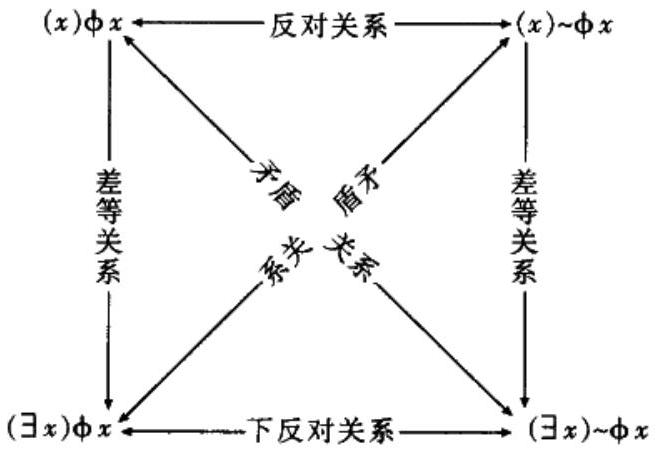
\includegraphics[width=\textwidth]{images/2025_05_15_6a28331d5e7c993ad07ag-463.jpg}

图10—1\\
继续假定至少存在一个个体,就该方阵我们可以说:\\
1.顶端的两个命题是反对关系;就是说,它们可以同时为假,但不能同时为真。

2.底端的两个命题是下反对关系;就是说,它们可以同时为真,但不能同时为假。

3.对角线相反两端的命题是矛盾关系;它们中一个为真,则另一个必定为假。

4.在方阵的每侧,下面命题的真被它正上方命题的真所蕴涵。

\begin{center}
\fbox{\parbox{0.95\textwidth}{
\textbf{本节要点}
\begin{itemize}
\item \textbf{从命题函项到命题的两种路径}:
  \begin{itemize}
  \item \textbf{列举方法}:用个体常元代入变元,产生关于特定个体的单称命题
  \item \textbf{概括方法}:通过量词约束变元,产生关于个体集合的普遍命题
  \item 体现了逻辑思维中从特殊到一般、从一般到特殊的双向运动
  \item 普遍命题具有非特指性、范围性、模式性、预测性等特征
  \end{itemize}
\item \textbf{全称量词的深入分析}:
  \begin{itemize}
  \item 符号$(x)$表示"对所有x都成立"
  \item \textbf{四大本质特征}:约束功能、普遍性、逻辑强度、可证伪性
  \item \textbf{哲学意义}:体现抽象能力、科学定律基础、理性追求、理论概括
  \item 一个反例就足以证伪全称陈述
  \end{itemize}
\item \textbf{存在量词的深入分析}:
  \begin{itemize}
  \item 符号$(\exists x)$表示"至少存在一个x使...成立"
  \item \textbf{四大本质特征}:存在承诺、弱逻辑强度、可验证性、开放性
  \item \textbf{认识论意义}:反映多样性认识、发现基础、可能性思维、假设框架
  \item 找到一个正例就足以验证存在陈述
  \end{itemize}
\item \textbf{量化命题的真值条件}:
  \begin{itemize}
  \item 全称量化为真当且仅当所有代入例都为真
  \item 存在量化为真当且仅当至少有一个代入例为真
  \item \textbf{存在假定}:至少存在一个个体的弱假定
  \item \textbf{重要关系}:$(x)Mx \rightarrow (\exists x)Mx$(从普遍到特殊)
  \end{itemize}
\item \textbf{否定在命题函项中的作用}:
  \begin{itemize}
  \item 扩展了命题函项概念,包括否定符"$\sim$"
  \item \textbf{四大重要性}:增强表达能力、量词转换基础、系统完整性、批判思维
  \item 为量词间的相互转换提供了基础
  \item 使逻辑系统更加完整和对称
  \end{itemize}
\item \textbf{量词对偶关系的深入分析}:
  \begin{itemize}
  \item \textbf{四组基本关系}:$\sim(x)\phi x = (\exists x)\sim\phi x$等
  \item 被称为\logicterm{德摩根定律的量词版本}
  \item 全称量词和存在量词是对偶的
  \item 任何量化陈述都可以用其对偶量词加否定来表达
  \end{itemize}
\item \textbf{量词逻辑方阵}:
  \begin{itemize}
  \item 描述全称肯定、全称否定、特称肯定、特称否定命题间的关系
  \item 包含反对关系、下反对关系和矛盾关系
  \item 展示量化命题间的逻辑蕴涵关系
  \item 为传统逻辑的现代化提供了精确的形式化工具
  \end{itemize}
\end{itemize}
}}
\end{center}